\section{Real-time implementation}

% agenda maybe changed a bit.

% fga, throughput and latency, accuracy
% benchmark, throughput
% demo or a picture.

\begin{frame}
    \frametitle{Implementation on Software-define Radio}

    \begin{figure}
        \centering
        \begin{minipage}{.5\textwidth}
          \centering
          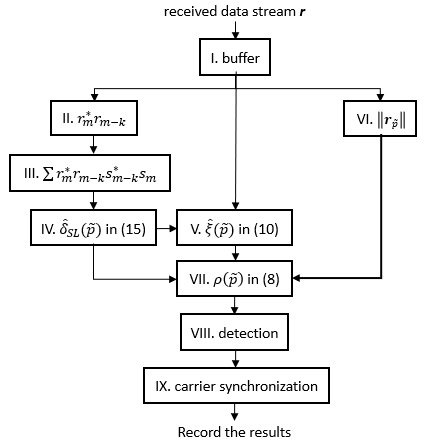
\includegraphics[width=.5\linewidth]{SDR_receiver_new.png}
        \end{minipage}%
        \begin{minipage}{.5\textwidth}
          \centering
          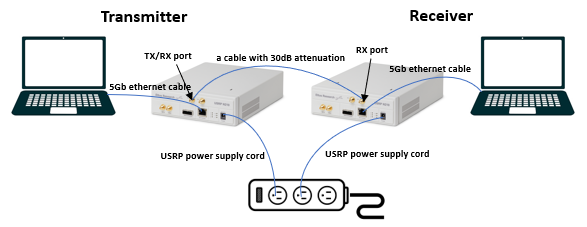
\includegraphics[width=.8\linewidth]{SDR_signal_transmission_path.png}
        \end{minipage}
    \end{figure}

    \begin{itemize}
        \item Different aspects of our algorithm are mapped to logical nodes in a pipelined, parallel processing architecture using Threading Building Blocks (TBB).
        \item The signals are transmitted and received between two universal software radio peripherals (USRP) connected by 5 Gb/s Ethernet cables to
        laptops.
        \item Accuracy, throughput and latency (the time when the first joint detection and estimation are finished) are considered. 
    \end{itemize}
  \end{frame}


  \begin{frame}
    \frametitle{Accuracy, throughput and latency}

    \begin{figure}
        \centering
        \begin{minipage}{.3\textwidth}
          \centering
          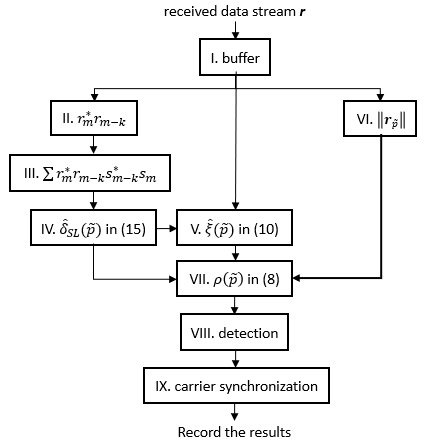
\includegraphics[width=.5\linewidth]{SDR_receiver_new.png}
        \end{minipage}%
        \begin{minipage}{.7\textwidth}
          \centering
          \begin{table}[t]
            \tiny
            \centering % used for centering table
            \begin{tabular}{c c c c} % centered columns (4 columns)
            \hline\hline %inserts double horizontal lines
            Node name & Time (ns) & CPU (ns) & Iterations \\ [0.5ex] % inserts table
            %heading
            \hline % inserts single horizontal line
            I. Buffer  & 3885 & 3885 & 200135 \\ % inserting body of the table
            II. $r_m^*r_{m-k}$  & 3252 & 3252 & 216211 \\
            III. $r_m^*r_{m-k}s_{m-k}^*s_m$ & 52343 & 52342 & 13388 \\
            IV. $\hat{\delta}_{SL}^{(1)}$ & 8432 & 8432 & 86480 \\
            V. $\hat{\xi}$ & 52309 & 52309 & 13359 \\
            VI. $||\bm{r}||$ & 19638 & 19638 & 34872 \\ % [1ex] adds vertical space
            VII. $\rho(p)$ & 16217 & 16217 & 42283 \\
            VIII. detection & 3669 & 3669 & 199976 \\
            IX. carrier synchronization & 3075 & 3075 & 222154  \\ [1ex]
            \hline
            \end{tabular}
            \label{table:BM_function_nodes} % is used to refer this table in the text
          \end{table}
        
        \end{minipage}
    \end{figure}

    \begin{itemize}
        \item Accuracy is checked by extracting one random received burst, correcting it with obtained phasor and frequency estimates and comparing with the training sequence.
        \item Use Google Benchmark to benchmark each computating cell and do tuning for the slowest cell to approach some throughput.
    \end{itemize}
  \end{frame}


  \begin{frame}
    \frametitle{Flow Graph Analyzer}

    \begin{figure}
        \centering
        \begin{minipage}{.3\textwidth}
          \centering
          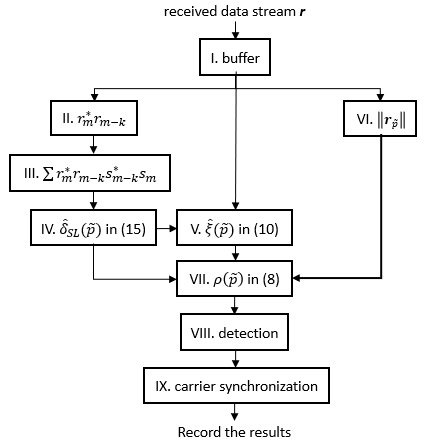
\includegraphics[width=.5\linewidth]{SDR_receiver_new.png}
        \end{minipage}%
        \begin{minipage}{.7\textwidth}
          \centering
          \begin{table}[t]
            \tiny
            \centering % used for centering table
            \begin{tabular}{c c c c} % centered columns (4 columns)
            \hline\hline %inserts double horizontal lines
            Node name & Time (ns) & CPU (ns) & Iterations \\ [0.5ex] % inserts table
            %heading
            \hline % inserts single horizontal line
            I. Buffer  & 3885 & 3885 & 200135 \\ % inserting body of the table
            II. $r_m^*r_{m-k}$  & 3252 & 3252 & 216211 \\
            III. $r_m^*r_{m-k}s_{m-k}^*s_m$ & 52343 & 52342 & 13388 \\
            IV. $\hat{\delta}_{SL}^{(1)}$ & 8432 & 8432 & 86480 \\
            V. $\hat{\xi}$ & 52309 & 52309 & 13359 \\
            VI. $||\bm{r}||$ & 19638 & 19638 & 34872 \\ % [1ex] adds vertical space
            VII. $\rho(p)$ & 16217 & 16217 & 42283 \\
            VIII. detection & 3669 & 3669 & 199976 \\
            IX. carrier synchronization & 3075 & 3075 & 222154  \\ [1ex]
            \hline
            \end{tabular}
            \label{table:BM_function_nodes} % is used to refer this table in the text
          \end{table}
        
        \end{minipage}
    \end{figure}

    \begin{itemize}
       \item Use flow graph analyzer (FGA) to 
    \end{itemize}
  \end{frame}